\chapter{Defining refactoring-oriented clone types}\label{chap:clonetypes}
In section \ref{chap:backgroundclonetypes} we introduced the four clone types as defined in literature. These simple definitions are suitable for analysis of a codebase. Their detection results in simple to understand numbers to argue about a codebase. However, these clone types have a few flaws which makes it hard to argue to what extend two fragments of code are functionally related. For each of type 1-3 clones~\cite{roy2007survey} we list our solutions to their shortcomings to increase the chance that we can refactor the clone while improving the design. Due to the serious challenges involved in their detection and refactoring, type 4 clones are not considered in this study.

We also look into clone detection tools for their suitability to support the proposed clone type definitions. We selected a few criteria  Most clone detection tools support these definitions of clone types. However, many of these tools use a vastly different approach. A study by Saini et al \cite{saini2018towards} outlines different clone detection tools and compares their results for each of type 1-3 clones. Even though they operate on the same type definitions, the tools used in this study yield different results.

\section{Shortcomings of clone types}
The clone definitions, as outlined in section \ref{chap:backgroundclonetypes}, allow reasoning about the duplication in a software system. Clones by these definitions can relatively easily and efficiently be detected. This has allowed for large scale analyses of duplication. However, these clone type definitions have shortcomings which makes the clones detected in correspondence with these definitions less valuable for (automated) refactoring purposes.

In this section we discuss the shortcomings of the different clone type definitions which make them less suitable for (automated) refactoring. Because of that, these clones require more judgement whether they should and can be refactored.

\subsection{Type 1 clones} \label{chap:type1clones}
Type 1 clones are \textit{identical clone fragments except for variations in whitespace and comments} \cite{roy2007survey}. This allows for the detection of clones that are the result of copying and pasting existing code, along with other reasons why duplicates might get into a codebase.

Type 1 clones are in most cases implemented as textual equality between code fragments (except for whitespace and comments). Although textually equal, method calls can still refer to different methods, type declarations can still refer to different types and variables can be of a different type. In such cases refactoring opportunities could be invalidated. An example of such a case is displayed in figure \ref{fig:type1}.

\begin{figure}[H]
  \includegraphics[width=1\columnwidth]{img/type1}
  \caption{Example of a type 1 clone.}
  \label{fig:type1}
\end{figure}

In the example in figure \ref{fig:type1}, we see a type 1 clone consisting of two methods. However, these clones might still be very hard to refactor as we cannot see by this example whether they are functionally equal. Both code fragments use different imported types, some of which imported via a wildcard. Because of this, it is hard to verify which of the used types have the same underlying implementation. This can make type 1 clones less suitable for refactoring purposes, as they require additional judgment regarding the refactorability of such a clone. When aiming to automatically refactor clones, applying refactorings to clones as shown in figure \ref{fig:type1}, is bound to be error prone and result in a uncompilable project or a difference in functionality.

Because of this, type 1 clones may not all be subject to refactoring. In section \label{chap:type1rclones} we describe an alternate approach towards detecting type 1 clones, which results in only clones that can be refactored.

\subsection{Type 2 clones}
Type 2 clones are \textit{structurally/syntactically identical fragments except for variations in identifiers, literals, types, layout and comments} \cite{roy2007survey}. This definition allows for the reasoning about code fragments that were copied and pasted, and then slightly modified. The two methods displayed in figure \ref{fig:type2} are type 2 clones of each other.

\begin{figure}[H]
  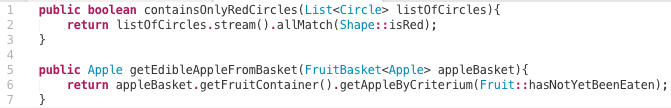
\includegraphics[width=1\columnwidth]{img/type2}
  \caption{Example of a type 2 clone.}
  \label{fig:type2}
\end{figure}

Looking at the example in listing \ref{fig:type2}, we see an example of a type 2 clone that poses no harm to the design of the system. Both methods are, except for their matching structure, completely different in functionality. They operate on different types, call different methods, return different things, etc. Having such a method flagged as a clone does not provide much useful information.

When looking at refactoring, type 2 clones can be very difficult to refactor. For instance if we have variability in types, the code can describe operations on two completely dissimilar types. Type 2 clones do not differentiate between primitives and objects, which makes the these clones often not so useful for refactoring purposes.

\subsection{Type 3 clones}
Type 3 clones are \textit{copied fragments with further modifications. Statements can be changed, added or removed in addition to variations in identifiers, literals, types, layout and comments} \cite{roy2007survey}. Detection of clones by this definition can be very hard, as it may be hard to detect whether a fragment was copied in the first place if it was severely changed. Because of this, most clone detection implementations of type 3 clones work on basis of a similarity threshold \cite{svajlenko2014evaluating, cordy2011nicad}. This similarity threshold has been implemented in different ways: textual similarity (for instance using levenshtein distance) \cite{lavoie2011automated}, token-level similarity of statement-level similarity.

Having a definition that allows for any change in code poses serious challenges on refactoring. A levenshtein distance of one can already change the meaning of a code fragment significantly, for instance if the name of a type differs by a character (and thus referring to different types).

\section{Refactoring-oriented clone types}
To resolve the shortcomings of clone types as outlined in the previous section, we propose alternative definitions for clone types to be directed at detecting clones that can and should be refactored. We have named these clones type 1R, 2R and 3R clones. These definitions share similarities with the literature definitions, the number of each type corresponds with the clone type it is modeled after. The ``R'' stands for refactoring-oriented (and may be less suitable for other analyses).

\subsection{Type 1R clones} \label{chap:type1rclones}
We propose an alternative definition of type 1 clones. This definition requires cloned fragments to be not just textually equal, but also functionally equal. Although requiring fragments to be functionally equal, type 1R clones do not allow for change in implementation (like type 4 clones). We check functional equality of two fragments by validating the equality of the fully qualified identifier for referenced types, methods and variables. Type 1R clones are a subset of type 1 clones.

\subsubsection{Referenced Types}
Many object-oriented programming languages (like Java, Python and C\#) require the programmer to import a type (or the class in which it is declared) before it can be used. Based on what is imported, the meaning of the name of a type can differ. For instance, if we import \texttt{java.util.List}, we get the interface which is implemented by all list datastructures in Java. However, importing \texttt{java.awt.List}, we get a listbox GUI component for the Java Abstract Window Toolkit (AWT). Because of this, for type 1R clones, we compare the fully qualified identifier for all referenced types.

\subsubsection{Called methods}
A codebase can have several methods with the same name. The implementation of these methods might differ. When we call two methods with an identical name, we can in fact call different methods. This is another reason that textually identical code fragments can differ functionally.

Because of this, for type 1R clones, we compare the fully qualified method signature for all method references. A fully qualified method signature consists of the fully qualified name of the method, the fully qualified type of the method plus the fully qualified type of each of its arguments. For instance, an \texttt{eat} method could become \texttt{com.sb.AppleCore com.sb.fruitgame.Apple.eat(com.sb.fruitgame.Tool)}.

\subsubsection{Variables}
In typed programming languages, each variable declaration should declare a name and a type. When we reference a variable, we only use its name. If, in different code fragments, we use variables with the same name but different types, the code can be functionally unequal but still textually equal. As an example, see the code in figure \ref{fig:type2variables}.

\begin{figure}[H]
  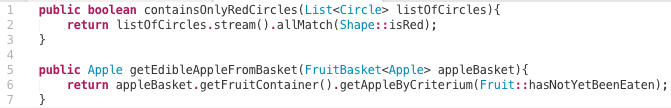
\includegraphics[width=1\columnwidth]{img/type2}
  \caption{Variables with different types but the same name.}
  \label{fig:type2variables}
\end{figure}

The body of both methods in figure \ref{fig:type2variables} is equal. However, their functionality is not. The first method adds two numbers together and the other concatenates an integer to a String.

For type 1R clones variable references should be compared by both type and name.

\subsection{Type 2R clones}
Type 2R clones are modelled after type 2 clones, which allow any change in identifiers, literals, types, layout, and comments. For refactoring purposes, this definition is unsuitable; if we allow any change in identifiers, literals, and types, we cannot distinguish between different variables, different types and different method calls anymore. This could render two methods that have an entirely different functionality as clones (as shown in figure \ref{fig:type2} previously). Refactoring such clones can be harmful instead of helpful.

We tackle these problems with type 2R clones to be able to detect such clones that can and should be refactored. Type 1R clones are a subset of type 2R clones. All rules that apply to type 1R clones also apply to type 2R clones. Additionally, type 2R clones allow variability in literals, variables and method calls. This variability however is constrained by a threshold. Type 2R do not allow any variability in types, as opposed to type 2 clones which do allow variability in types. As type 2R clones are per definition more permissive than type 1R clones, type 1R clones are a subset of type 2R clones.

\subsubsection{A threshold for variability in literals, variables and method calls}
Type 2 clones allow any variability in literals, variables and method identifiers. However, this information tells a lot about the meaning of the code fragment. Most clone detection tools do not differentiate between a type 2 clone that differs by a single literal/identifier and one that differs by many. However, this does have a big impact on the meaning of the code fragment and thus the harmfulness of the duplication being there.

For type 2R clones we define a threshold for variability in literals, variables and method calls. We calculate the variability in literals, variables and method calls using the following formula:

$$T2R\ Variability\ Percentage=\frac{Diff(l) + Diff(v) + Diff(m)}{Total(t)}*100$$
$$Diff=Amount\ that\ differ\ from\ other\ clone\ instances\ in\ the\ clone\ class$$
$$Total\ =\ Total\ number\ in\ the\ clone\ instance$$
$$l=Number\ of\ literals$$
$$v=Number\ of\ variables$$
$$m=Number\ of\ method\ calls$$
$$t=Number\ of\ tokens$$

\paragraph{Literal and variable variability}
We allow only variability in the value of literals and variables, but not in their types. This is because a difference in literal/variable type may have a big impact on the refactorability of the cloned fragment. When we refactor different literals/variables that have both the same type, in case of an ``Extract Method'' refactoring, we have to create a parameter for this literal and pass the corresponding literal/variable from cloned locations. However, if two literals have different types, this might not be possible (or will have a negative effect on the design of the system). This is because a lot of variability in literals will result in more parameters required in the extracted method, which is detrimental for the design of the system.

Consider the example in figure \ref{fig:type2literal}. In this example, the two methods have two literals that differ between them. We can perform an ``Extract method'' refactoring on these to get the result that is displayed on the right. In this process, we create a method parameter for the corresponding literal.

\begin{figure}[H]
  \centering
  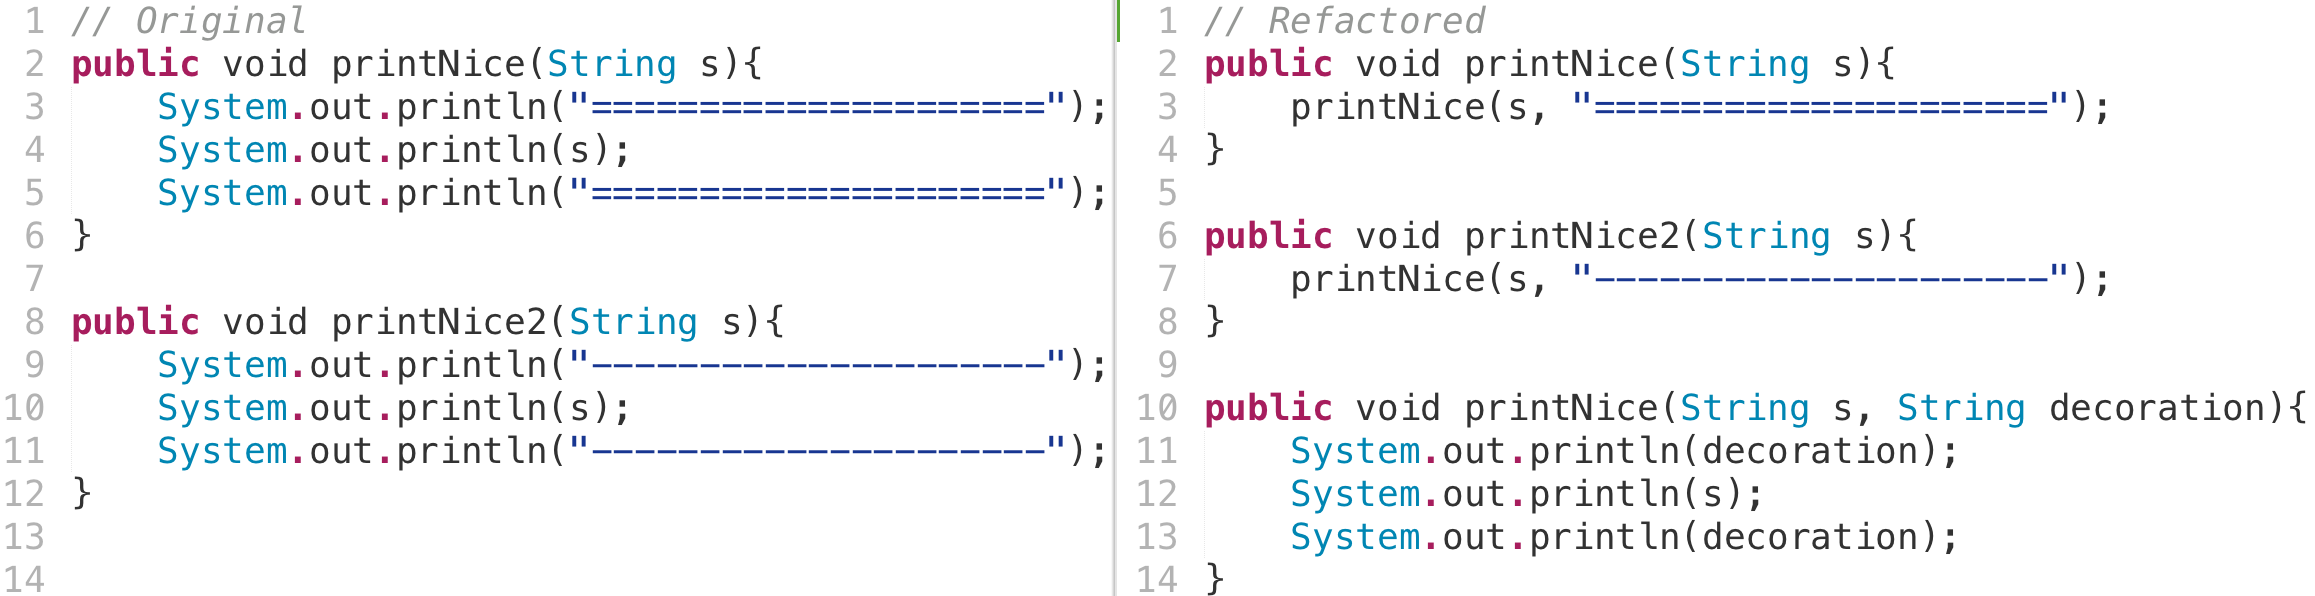
\includegraphics[width=1\columnwidth]{img/type2literal}
  \caption{Literal variability refactored.}
  \label{fig:type2literal}
\end{figure}

\paragraph{Method call variability}
Most modern programming languages (like Java, Python and C\#) allow to pass method references as a parameter to a method. This helps reducing duplication, as it is possible to refactor two code fragments which differ only by a method call. However, a method call does often not consist of a single token (like variables and literals). For instance, a method call \texttt{System.out.println()} consists of several segments: a type reference to the \texttt{System} type, a reference to the static \texttt{out} field and a call of the \texttt{println()} method.

For type 2R clones, we allow called methods to vary as long as they have the same argument types and return type (both of them should be compared using their fully qualified identifiers). An example of this is shown in figure \ref{fig:type2method}. In this example, we have two methods (\texttt{System.out.println} and \texttt{myFancyPrint}). We use the ``Extract Method'' refactoring method to extract a new method and use a parameter for to pass the used method.

The method call variability property of type 2R clones imply that type 2R clones are not a subset of type 2 clones. Because methods calls can have a different structure, type 2R clones can be structurally slightly different. The example as shown in figure \ref{fig:type2method} can be a type 2R clone (dependent on the thresholds used), but is not a type 2 clone.

\begin{figure}[H]
  \centering
  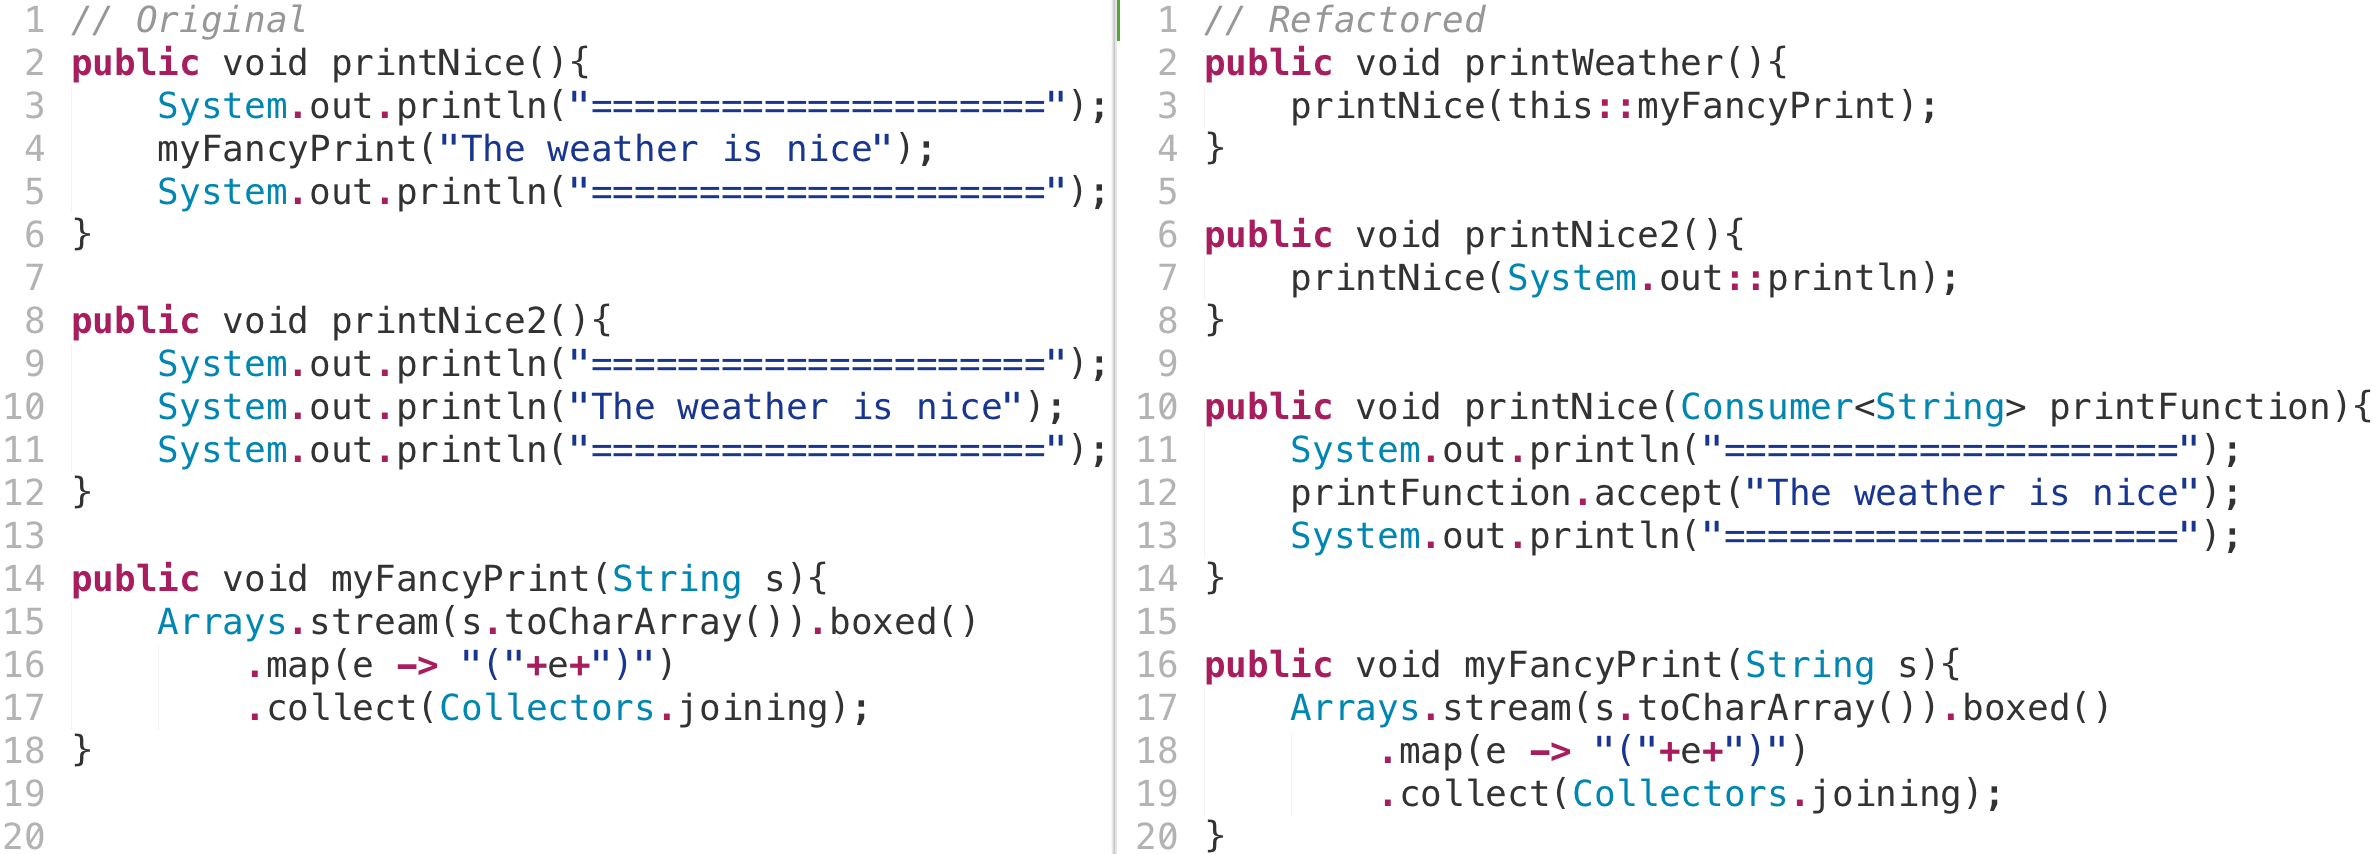
\includegraphics[width=1\columnwidth]{img/type2method}
  \caption{Method variability refactored.}
  \label{fig:type2method}
\end{figure}

\subsubsection{Allow any change in method and class names}
When refactored, some identifiers have no detrimental effect on the design if they vary between cloned instances. In the previous section, variability in literals, variables and called methods would result in more parameters for the extracted method, thus indicating a detrimental effect on system design. This is not the case with the name of a method declaration and the name of a class/interface/enumeration declaration.

If a full method is cloned with another method, however only their names differ, we can refactor these methods to keep only one of them. Allowing any change in method and class names will only indicate a refactoring opportunity if the full method or class is cloned.

\section{Type 3R clones}
Type 3 clones allow any change in statements, often bounded by a similarity threshold. This means that type 3R allows the inclusion of a statement that is not detected by type 1 or 2 clone detection. When looking at how we can refactor a statement that is not included by one clone instance but is in another, we find that we require a conditional block to make up for the difference in statements. See figure \ref{fig:type3} for an example of such a clone.

\begin{figure}[H]
  \centering
  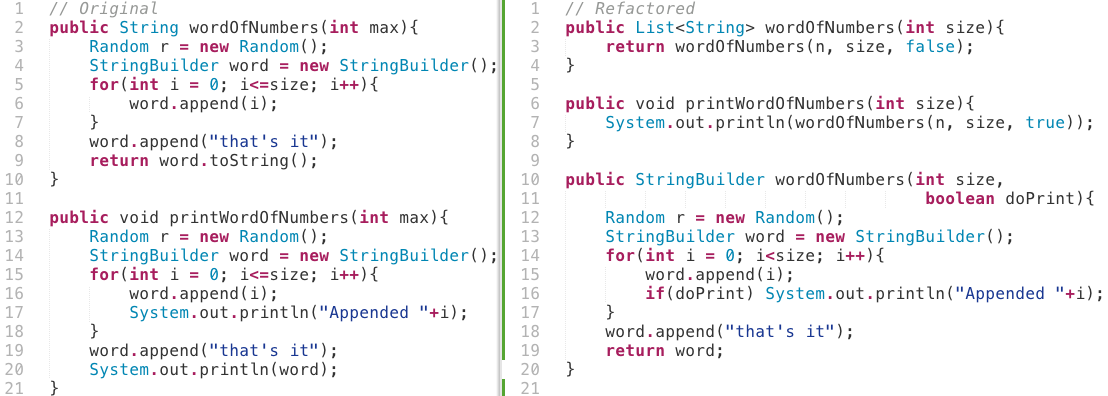
\includegraphics[width=1\columnwidth]{img/type3_3}
  \caption{Added statement between cloned methods.}
  \label{fig:type3}
\end{figure}

In figure \ref{fig:type3} a single statement is added. This statement is found in between cloned lines. We have named this difference between the two clones, in this examples containing a single statement, the \textit{gap}. This gap has a threshold for type 3R, which is calculated by the following formula:

$$T3R\ Gap\ Percentage=\frac{Statements(C_{gap})}{Statements(C_{above} \cup C_{below})}*100$$
$$Statements = The\ amount\ of\ statements\ in\ this\ code\ fragment$$
$$C_{gap} = The\ gap between two clones$$
$$C_{above} = The\ clone\ instance\ above\ the\ gap$$
$$lower = The clone instance below the gap$$

Apart from this threshold, the gap in between clones may not span over different blocks. Look at figure \ref{fig:type3invalid} for an example of this. We cannot refactor both statements into a single conditional block. We could however use two conditional blocks, but due to the detrimental effect on the design of the code (as each conditional block adds a certain complexity), we decided not to allow this for type 3R clones.

\begin{figure}[H]
  \centering
  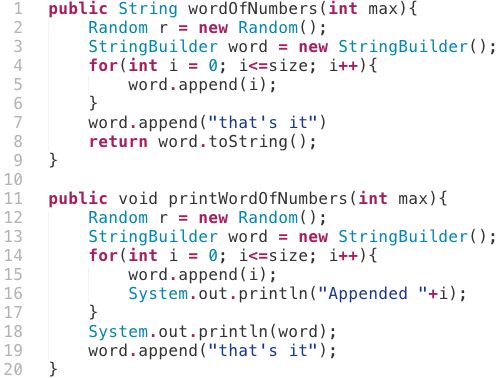
\includegraphics[width=0.6\columnwidth]{img/type3invalid}
  \caption{Statements between clones in different blocks.}
  \label{fig:type3invalid}
\end{figure}

\section{The challenge of detecting these clones}\label{chap:challenge}
To detect each type of clone, we need to parse the fully qualified identifier of all types, method calls and variables. This comes with serious challenges, regarding both performance and implementation. Also, to be able to parse all fully qualified identifiers, and trace the declarations of variables, we might need to follow cross file references. The referenced types/variables/methods might even not be part of the project, but rather of an external library or the standard libraries of the programming language. All these factors need to be considered for the referenced entity to be found, on basis of which a fully qualified identifier can be created.

Mainly the requirement to have access to all external libraries is a difficult one to satisfy in diverse projects. Because of this, the proposed clone definitions may be less suitable for large scale clone detection purposes.

\section{Unifying the types}\label{sec:unifying}
In this chapter we have proposed refactoring-oriented definitions using the type 1, 2 and 3 clone definitions from literature as a baseline. In literature, these definitions are mainly aimed towards reasoning about duplication in source code. When considering these types for refactoring, the goal becomes slightly different. Because of this, having separate clone type definitions does not have any value. Rather, we need a single clone type definition by which we can detect all clones that can and should be considered for refactoring.

Because of this, the ultimate goal would be not to consider type 1R, 2R and 3R separately, but together. However, this is dependent on good thresholds for the type 2R variability and type 3R gap size. Because of this, we have dedicated section \ref{sec:thresholds} to performing measurements to find good thresholds. The ultimate goal is to have a single unified definition of clones that can and should be refactored. Although it will be next to impossible to define such a definition and its corresponding thresholds that does not detect false positives. However, we strive to find at least a near-optimal set of thresholds regarding the type definitions proposed in this chapter.

\section{Suitability of existing Clone Detection Tools for detecting these clones}
\label{ch:tool-overview}
We conducted a short survey on (recent) clone detection tools in order to expand them with the proposed types. The results of our survey are displayed in table~\ref{table:dettools}. We chose a set of tools that are open source and can analyze at least one popular object-oriented programming language. Next, we formulate the following four criteria by which we analyze these tools:
\begin{enumerate}
    \item \textbf{Should find clones in any context.} Some tools only find clones in specific contexts, such as only method-level clones. We want to perform an analysis on all clones in projects to get a complete overview. We analyzed this behavior using a set of control projects.
\item \textbf{TODO: Criterium.}\simon{TODO} We assembled a number of test projects to assess the validity of clone detection tools. On basis of this, we checked whether clone detection tools can correctly find clones in diverse contexts.
\item \textbf{Can analyse resolved symbols.} When detecting clones for refactoring purposes, it is important that clone instances can be refactored. Sometimes, textual equality between code fragments does not imply that these can be refactored (this is described more elaborately in section \ref{chap:type1clones}). Because of this, we want to use a clone detection tool that can analyze such structures.
\item \textbf{Extensive detection configuration.} We aim to exclude expressions/statements from matching (more about our rationale in section~\ref{chap:clonetypes}). To achieve this, the tool needs to be able to allow those threshold changes. This can be either through simple changes of the source code, or by using some configuration file.
\end{enumerate}

\begin{table}[H]
 \begin{center}
  \caption{Our survey on clone detection tools.} \label{table:dettools}
  \medskip
\begin{tabular}{|l|l|l|l|l|l|}
\hline
\textbf{Clone Detection Tool} & \textbf{(1)} & \textbf{(2)} & \textbf{(3)} & \textbf{(4)} \\ \hline
Siamese \cite{ragkhitwetsagul2019siamese} &  &             &             & \checkmark            \\ \hline
NiCAD \cite{roy2008nicad, cordy2011nicad} & \checkmark                             & \checkmark            &             &             \\ \hline
CPD \cite{roy2009comparison} & \checkmark & \checkmark            &             &             \\ \hline
\begin{tabular}[c]{@{}l@{}}CCFinder \cite{kamiya2002ccfinder}\\ D-CCFinder \cite{livieri2007very}\end{tabular} & \checkmark  & \checkmark   &    &   \\ \hline
CCFinderSW \cite{semura2017ccfindersw}   &    &             &             & \checkmark            \\ \hline
\begin{tabular}[c]{@{}l@{}}SourcererCC \cite{sajnani2016sourcerercc}\\ Oreo \cite{saini2018oreo}\end{tabular} & \checkmark    &             &             & \checkmark            \\ \hline
BigCloneEval \cite{svajlenko2016bigcloneeval}  & \checkmark  & \checkmark   &             &             \\ \hline
Deckard \cite{jiang2007deckard} & \checkmark   &             & \checkmark            &             \\ \hline
Scorpio \cite{higo2013revisiting, kamalpriya2017enhancing} & \checkmark   &     & \checkmark  & \checkmark   \\ \hline
\end{tabular}
\end{center}
\end{table}

None of the state-of-the-art tools we identified implement all our criteria, so we decided to implement our own clone detection tool, which is further described in the next chapter.

\chapter{Evaluation setup}
In this chapter we describe the setup we use for our experiments. Our most prominent contribution is the proposal of a tool called CloneRefactor. This tool allows us to map clones with all clone definitions as described in chapter \ref{chap:clonetypes}.

All results of our experiments, as displayed in chapter \ref{ch:results}, are measured over a corpus of Java projects. In this chapter we will explain how we prepared this corpus.

\section{CloneRefactor}
CloneRefactor is the name of our clone detection and refactoring tool. It features the following novel functions:
\begin{itemize}
  \item Detection of clone classes rather than clone pairs.
  \item A novel detection method, aimed at extensibility.
  \item Detection of refactoring-oriented clone types, in addition to the literature clone types.
  \item Allows for automated refactoring of a subset of the detected duplication issues.
\end{itemize}
In this section we describe our approach and rationale for the design decisions regarding this tool.

\begin{figure}[H]
  \centering
  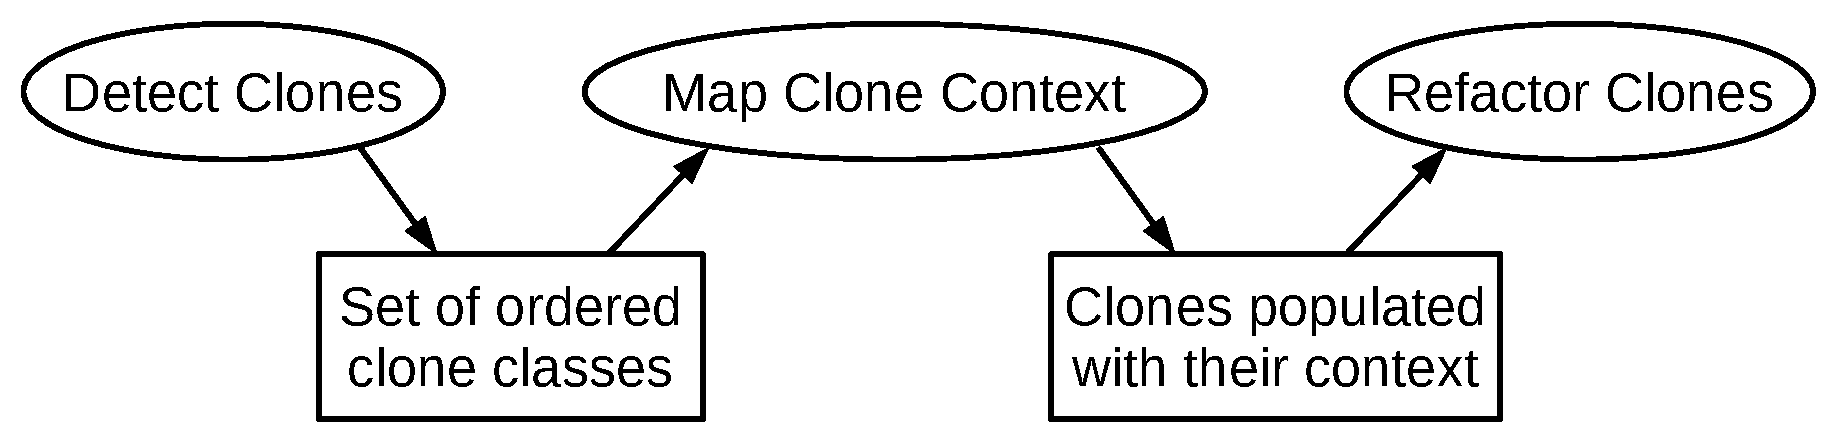
\includegraphics[width=0.8\columnwidth]{img/CloneRefactorOverall}
  \caption{CloneRefactor overall process.}
  \label{fig:clonerefactorprocess}
\end{figure}

Figure \ref{fig:clonerefactorprocess} shows the overall process used by CloneRefactor. First, we detect clones on basis of a Java codebase, given a Java project from disk and a configuration. The clone detection process is further explained in section \ref{sec:clonedetection}. After all clones are found, CloneRefactor maps the context of the clones. On basis of this context, CloneRefactor applies transformations to the source code for clones for which we have configured a refactoring.

\subsection{JavaParser}
A very important design decision for CloneRefactor is the usage of a library named JavaParser \cite{tomassetti2017javaparser}. JavaParser is a Java library which allows to parse Java source files to an abstract syntax tree (AST). JavaParser allows to modify this AST and write the result back to Java source code. This allows us to apply refactorings to the detected problems in the source code.

Integrated in JavaParser is a library named SymbolSolver. This library allows for the resolution of symbols using JavaParser. For instance, we can use it to trace references (methods, variables, types, etc) to their declarations (these referenced identifiers are also called ``symbols''). This is very useful for the detection of our refactoring-oriented clone types, as they make use of the fully qualified identifiers of symbols.

In order to be able to trace referenced identifiers SymbolSolver requires access to not only the analyzed Java projects, but also all its dependencies. This requires us to include all dependencies with the project. Along with this, SymbolSolver solves symbols in the JRE System Library (the standard libraries coming with every installation of Java) using the active Java Virtual Machine (JVM). This has a big impact on performance efficiency.

Because of the requirement of symbol resolution, the refactoring-oriented clone types are less suitable for large scale clone analysis.

\subsection{Clone Detection}\label{sec:clonedetection}
To detect clones, CloneRefactor parses the AST aqcuired from JavaParser to an unweighted graph structure. On basis of this graph structure, clones are detection. Dependent on the type of clones being detected, transformations may be applied. The way in which CloneRefactor was designed does not allow for several clone types to be detected simultaneously, in accordance with our clone type philosophy as described in chapter \ref{sec:unifying}.

The overall process regarding clone detection is displayed in figure \ref{fig:clonedetection}. First of all, we use JavaParser to read a project from disk and build an AST, one class file at a time. Each AST is then converted to a grid that maps relations between statements, further explained in section \ref{sec:clonegrid}. On basis of this grid, we detect clone classes and verify them using three thresholds (in order of importance):
\begin{itemize}
  \item Amount of tokens.
  \item Amount of statements.
  \item Amount of lines.
\end{itemize}
If the detection was configured to detect either type 2R, 3 or 3R clones we perform some type specific transformations on the resulting set of clones.

\begin{figure}[H]
  \centering
  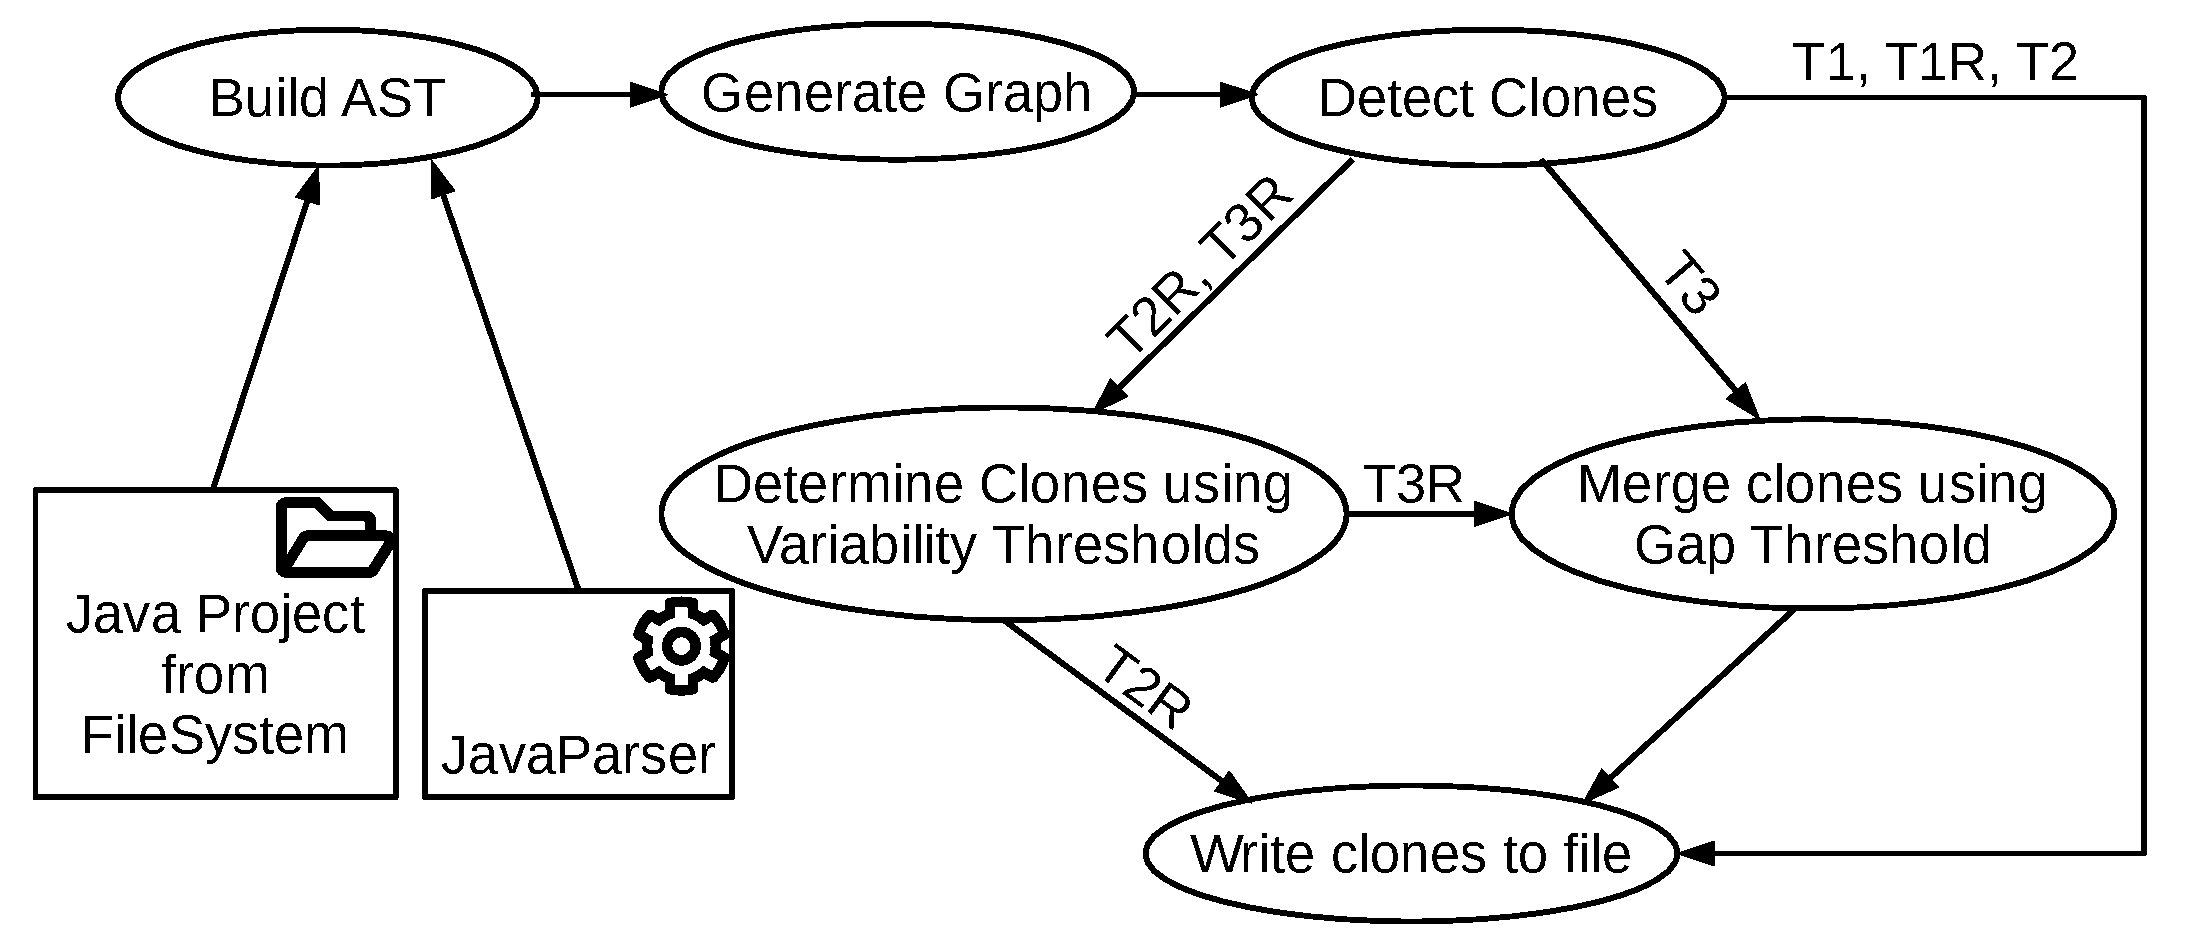
\includegraphics[width=1\columnwidth]{img/CloneDetection}
  \caption{CloneRefactor clone detection process.}
  \label{fig:clonedetection}
\end{figure}

\subsubsection{Generating the clone grid}\label{sec:clonegrid}
First of all, we parse the AST obtained from JavaParser into what we call a clone grid. Although it is not a grid in an original sense, thinking of it as a grid makes it easier to comprehend (this is explained in section \ref{sec:detectingclones} in more detail). We have chosen to base our clone detection around statements as the smallest unit of comparison. This means that a single statement cloned with another single statement is the smallest clone we can find. The rationale for this lies in both simplicity and performance efficiency. This means we won't be able to find when a single expression matches another expression, or even a single token matching another token. This is in most cases not a problem, as expressions are often small and do not span the minimal size to be considered a clone in the first place (more about this in section \ref{sec:thresholds}).

Building the ``clone grid'' consists of walking the AST in-order for each declaration and statement. For each declaration/statement found, we map the following relations:
\begin{itemize}
  \item The declaration/statement preceding it.
  \item The declaration/statement following.
  \item The last \textbf{preceding} declaration/statement with which it is cloned.
\end{itemize}
We do not create a separate grid for each class file, so the statement/declaration preceding or following could be in a different file. While mapping these relations, we maintain a hashed map containing the last occurrence of each unique statement. This map is used to quickly find out whether a statement is cloned with another. An example of such a grid is displayed in figure \ref{fig:clonegridsimple}.

\begin{figure}[H]
  \centering
  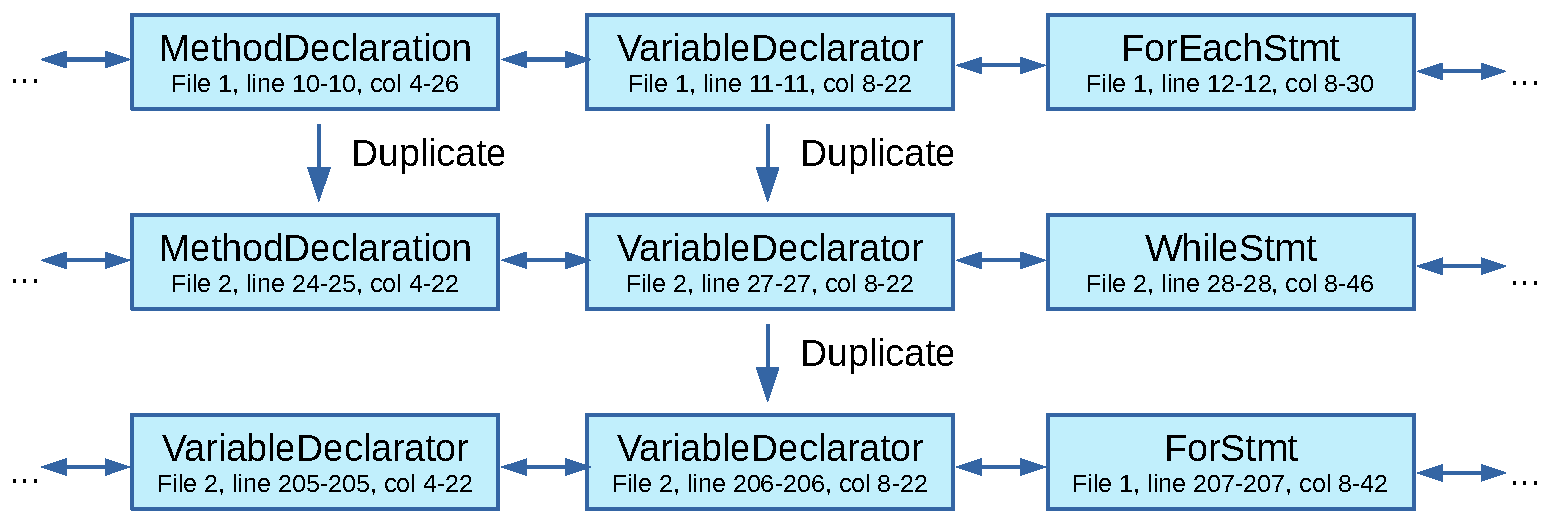
\includegraphics[width=1\columnwidth]{img/CodeGraph2}
  \caption{Clone grid as built by CloneRefactor.}
  \label{fig:clonegridsimple}
\end{figure}

We generally call the declarations and statements represented in this grid \textit{nodes}. The relations \textit{next} and \textit{previous} in this grid are represented as an undirected relation. The relations representing duplicated are directed. This is a restriction we've chosen as it creates an important constraint for the clone detection process. This process is explained in section \ref{sec:detectingclones}.

\subsubsection{Comparing Statements/Declarations}
In the previous section we described a ``duplicate'' relation between nodes in the clone grid built by CloneRefactor. Whether two nodes in this grid are duplicates of each other is dependent on the clone type. In this section, we will describe for each type how we compare statements and declarations assess whether they are clones of each other.

CloneRefactor detects six different types of clones: T1, T2, T3, T1R, T2R and T3R. These types are further explained in chapter \ref{chap:clonetypes}. For \textbf{type 1} clones, CloneRefactor filters the tokens of a node to exclude its comments, whitespace and end of line (EOL) characters and then compares these tokens. For \textbf{type 2} clones, the tokens are further filtered to omit all identifiers and literals. \textbf{Type 3} clones do the same duplication comparison as type 2 clones.

For \textbf{type 1R} clones, this comparison is a lot more advanced. For \textit{method calls} we trace their declaration and use its fully qualified method signature for comparison with other nodes. For all \textit{referenced types} we trace their declarations and use assemble their fully qualified identifier for comparison with other nodes. For \textit{variables} we trace their declaration and their types. If the variable type is a primitive we can directly use it for comparison. If it is a referenced type, we have to trace this type first in order to collect their fully qualified identifier for comparison.

For \textbf{type 2R} clones we allow any variation in literals, variables and method calls at this stage in the clone detection process. However, for \textit{literals} we do resolve their type in order to verify that they are of the same type. For \textit{variables} we also only verify that their types are the same (but not their names). For \textit{method calls}, we trace their declaration but only compare the fully qualified identifier for its return type and each of its arguments' types. Apart from that, we do not compare the names of method, class, interface and enum declarations.

In this stage, \textbf{type 3R} clones have the same compare rules as type 2R clones.

\subsubsection{Detecting Clones} \label{sec:detectingclones}
After building the clone grid, we use it to detect clones. We decided to focus on the detection of clone classes rather than clone pairs because clone pairs do not provide a general overview of all entities containing the clones, with all their related issues and characteristics \cite{fontana2012duplicated}. Although clone classes are harder to manage, they provide all information needed to plan a suitable refactoring strategy, since this way all instances of a clone are considered. Another issue that results from grouping clones by pairs: clone reference amount increases according to the binomial coefficient formula (two clones form a pair, three clones form three pairs, four clones form six pairs, and so on), which causes a heavy information redundancy \cite{fontana2012duplicated}.

As stated in the previous section, nodes in the grid link to \textit{preceding} cloned statement. This implies that the first node that is cloned does not have any clone relation, as there are no clones preceding it (only following it). Because of this, we start our clone detection process at the final location encountered while building the grid. For this node, we collect all nodes it is cloned with. Even though the final node only links to the preceding node it is cloned with, we can collect all clones. This is because the preceding clone also has a preceding clone (if applicable) and we can follow this trail to collect all clones of a single node. As an example, see figure \ref{fig:clonegrid}.

\begin{figure}[H]
  \centering
  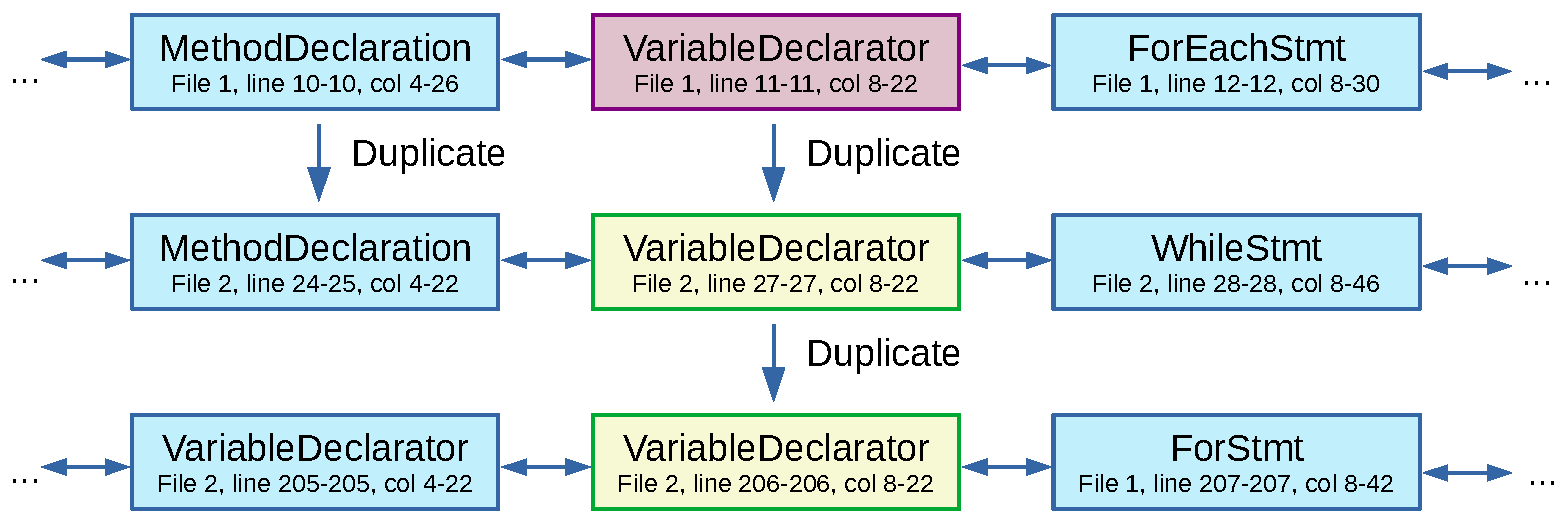
\includegraphics[width=1\columnwidth]{img/CodeGraph3}
  \caption{Clone grid with a clone class consisting of three clone instances marked.}
  \label{fig:clonegrid}
\end{figure}

Using the example shown in figure \ref{fig:clonegrid} we can explain how we detect clones. Suppose we are finding clones for two files and the final node of the second file is a variable declarator. This final node is represented in the example figure by the purple box (1). We then follow all ``duplicate'' relations until we have found all clones (2 and 3). We now have a single statement clone class of three clone instances (1, 2 and 3). Next, we move to the previous line (4). Here again, we collect all duplicates of this node (4 and 5). For each of these duplicates, we check whether the node following it is already in the clone class we collected in the previous iteration. In this case, (2) follows (5) and (1) follows (4). This means that node (3) does not form a `chain' with other cloned statements. Because of this, the clone class of (1, 2 and 3) comes to an end. It will be checked against the thresholds, and if adhering to the threshold, considered a clone. We then go further to yet the previous node (6). In this case, this node does not have any clones. This means we check the (2 and 5, 1 and 4) clone class against the thresholds, and if it adheres, consider it a clone. Dependent on the thresholds, we'd now have found two clone classes.

The grid representation shown in figure \ref{fig:clonegrid} is only shown as a grid for ease of comprehension. In fact, it is not a grid, but a graph. Eventually, following only the ``previous node'' relations, we can get from (6) to (2). When we are at that point, we will find only one cloned node for (2), namely (3). However, after we check this clone against the thresholds, we check whether it is a subset of any exisiting clone. If this is the case, we discard the clone.

\subsubsection{Validating the type 2 variability threshold}

\subsubsection{Checking for type 3 opportunities}


\section{The corpus}\label{chap:corpus}
For our measurements we use a large corpus of open source projects \cite{githubCorpus2013}. This corpus has been assembled to contain relatively higher quality projects. Also, any duplicate projects were removed from this corpus. This results in a variety of Java projects that reflect the quality of average open source Java systems and are useful to perform measurements on.

As indicated in chapter \ref{chap:challenge} CloneRefactor requires all libraries of software projects we test. As these are not included in the used corpus \cite{githubCorpus2013}, we decided to filter the corpus to only include Maven projects. Maven is a build automation tool used primarily for Java, and works on basis of an \texttt{pom.xml} file to describe the projects' dependencies. As no \texttt{pom.xml} files are included in the corpus, we cloned the latest version of each project in the corpus. We then removed each project that has no \texttt{pom.xml} file. As a final step, we collected all dependencies for each project by using the \texttt{mvn dependency:copy-dependencies -DoutputDirectory=lib} Maven command, and removed each project for which not all dependencies were available (due to non-Maven dependencies being used or unsatisfiable dependencies being referenced in the \texttt{pom.xml} file).

Some general data regarding this corpus is displayed in Table \ref{table:general}.

\begin{table}[H]
  \begin{center}
  \caption{General results for GitHub Java projects corpus \cite{githubCorpus2013}.} \label{table:general}
  \medskip
\begin{tabular}{|l|l|}
\hline
Amount of projects                                                                                      & 1,361      \\ \hline
\begin{tabular}[c]{@{}l@{}}Amount of lines (excluding\\whitespace, comments and newlines.)\end{tabular} & 1,414,996  \\ \hline
Amount of statements/declarations                                                                       & 1,212,189  \\ \hline
\begin{tabular}[c]{@{}l@{}}Amount of tokens (excluding\\whitespace, comments and newlines.)\end{tabular} & 11,643,194 \\ \hline
\end{tabular}
\end{center}
\end{table}
